% commands often have optional arguments that can be set using square brackets and keywords
% this sets the font size to be 11, a4 paper size, and the text in two columns
\documentclass[11pt, a4paper, twocolumn]{article}


\usepackage{graphicx} % Required for inserting images
\usepackage{lipsum}
\usepackage{amsmath}

% the geometry package allows us to set the margins manually
% \usepackage[margin=2.5cm]{geometry} % set them uniformly
% or set each one independently
\usepackage[
    top=2cm,
    left=2cm,
    right=2cm,
    bottom=2cm,
]{geometry}


% the rest of this example is the sme as 01-mwe.tex

\title{LaTeX Tutorial}
\author{Jeremy Worsfold}
\date{June 2025}


%import your packages before you begin the document
\begin{document}

\maketitle

\section{Introduction}

I can type sentences and paragraphs just by typing.
A new line doesn't do anything really but it helps you see your text easier and track changes better.
I like to start a new line for each sentence.

A blank line, however, does start a new paragraph. You can force line breaks with double backslashes but I wouldn't advise this. 
Be careful with some special characters when typing such as ampersands, percentage, dollar, at symbol etc. To show these as text, use a backslash before: \%, \$, \&, \$. But these shouldn't come up regularly anyway.
For single quotation marks, use `at the start and' at the end. For double quotes, use ``and''. 
If you didn't, the left one would look "weird".


\section{Typesetting maths}

You can add maths inline using $x=mx + b$, or \(x=mx+b\). You can put it on its own line using 
\[
    A\Sigma + \Sigma^T A = B
\]
But I typically use an equation \textit{environment}
\begin{equation}
    \int_{-\infty}^\infty e^{-x^2} d x = \sqrt{\pi}
\end{equation}
Or the same way but not with numbering
\begin{equation*}
    \int_{-\infty}^\infty e^{-ax^2} d x = \sqrt{\frac{\pi}{a}}
\end{equation*}

Importing other packages can bring other ways of typesetting maths, eg the \texttt{amsmath} package brings the \texttt{align} environment, which works the same way but also allows you to split equations across multiple lines
\begin{align}
    \sin(2\theta) & = 2\cos(\theta)\sin(\theta) \\
    & = 1-2\cos^2(\theta).
\end{align}
The double backslash starts a new line and the ampersands are the anchor points for each line.
For more information on breaking across multiple lines and and different ways of numbering, look up and have a go with other environments.
For example, using \texttt{subequations, align}:
\begin{subequations} % number equations with a,b etc
\begin{align} % allow equations to go over multiple lines
    \sin(2\theta) & = 2\cos(\theta)\sin(\theta) \\
    & = 1-2\cos^2(\theta).
\end{align}
\end{subequations}

Using \texttt{equation, aligned}:
\begin{equation} % number equations with a,b etc
\begin{aligned} % allow equations to go over multiple lines
    \sin(2\theta) & = 2\cos(\theta)\sin(\theta) \\
    & = 1-2\cos^2(\theta).
\end{aligned}
\end{equation}

\begin{figure}
    \centering
    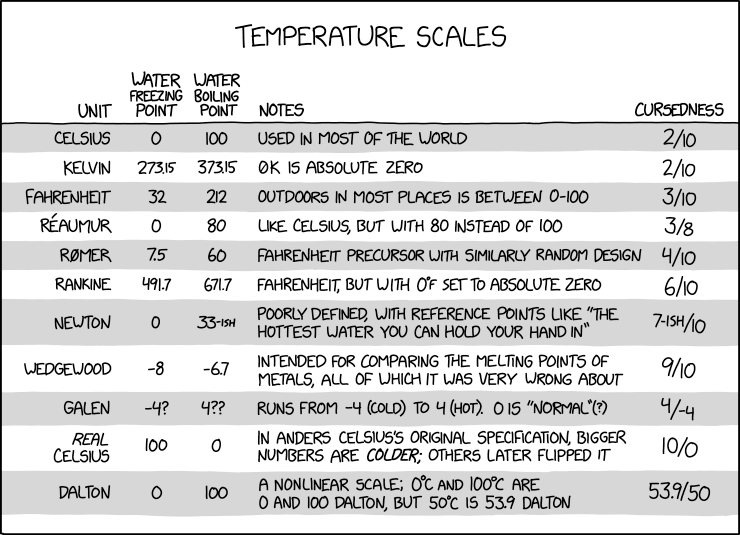
\includegraphics[width=\linewidth]{figures/temperature_scales.png}
    \caption{Caption}
    \label{fig:temp-scales}
\end{figure}

\subsection{Lipsum}

\lipsum

\end{document}
